\documentclass[12pt]{article}
\usepackage{amsmath}
\usepackage{amssymb}
\usepackage{graphicx}
\usepackage{comment}
\usepackage{longtable}
\usepackage{graphicx}

\begin{document}

\title{\textbf{SOFTWARE ARCHITECTURE DOCUMENT }}
\maketitle

\begin{center}
\title{\textbf{Software Design COMS3009}}
\maketitle
\end{center}
\begin{center}
\title{\textbf{FindMeTutor Android Application}}
\maketitle
\end{center}

\begin{center}
Proposed idea by:\\
Shaneel James-718840
\\Jadon Manilal-815050
\\Jared Naidoo - 719238
\\Krupa Prag - 782681
\\Nivek Ranjith - 802119
\end{center}


\newpage
%TABLE OF CONTENTS
\tableofcontents
\newpage


\section{\textbf{Introduction}}
%\begin{flushleft}
\begin{itemize}

\item Purpose\\
The Software Architecture Document (SAD) provides a comprehensive architectural overview of the FindMeTutor system. It presents a number of different architectural views to depict different aspects of the system. It is intended to capture and depict the different architectural decisions which have been made on the system.

\item Scope\\
The scope of the SAD is to depict the architecture of the FindMeTutor. This includes the FindMeTutor tutor application, FindMeTutor student application and the database (backend systems) which allow FindMeTutor to operate.

\item Definitions, Acronyms and Abbreviations\\
UML: Unified Modeling Language\\
SAD: Software Architecture Document
\end{itemize}

%\end{flushleft}
\pagebreak

\section{Architecture}
This section contains a description pertaining to the architecture used in the FindMeTutor system.

\begin{itemize}
\item Type of Architecture\\
The FindMeTutor system makes use of a 2 tier architecture. The application layer contains the user-interface and business logic. The second layer is the database ,which contains the user data for the system. Below is a diagram which depicts the architecture selected:\\
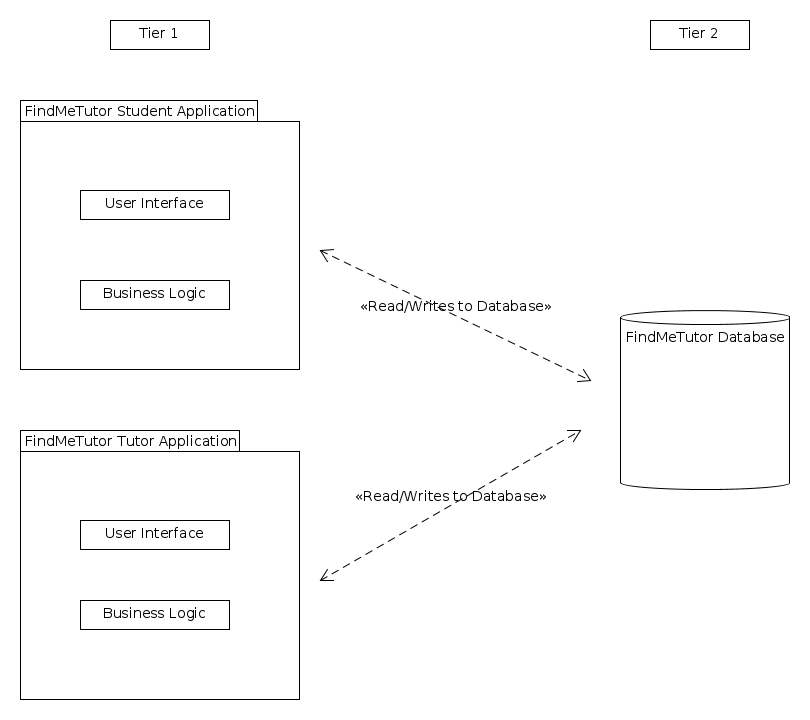
\includegraphics[width=140mm]{./2_Tier_Diagram.png}\\

\item Advantages
\begin{itemize}
\item Allows the application to be easily devloped due to simplicity.
\item Maximum user satisfaction can be ensured due to accurate and fast prototyping of applications
\item Database logic and business logic is physically close, which offers higher performance.\\
\end{itemize}

\item Responsibilities of Layer 1:
\begin{itemize}
\item Contains the businnes logic and user interface all built into the application. The first layer is responsible for all actions with the client. Contains the administration layer used to add funds to a student/tutor account as well as general configuration.
\end{itemize}

\item Responsibilities of Layer 2:
\begin{itemize}
\item Contains the data for the system.Allows multiple users to access the same data simultaneously.
\end{itemize}

\item Systems of interest\\
The main systems of interest are the FindMeTutor which contain the following two subsystems:
\begin{itemize}
\item FindMeTutor Student Application
\item FindMeTutor Tutor Application
\end{itemize}

\item Supplementary Information\\
The FindMeTutor system comprises of two main components: The FindMeTutor student application and the FindMeTutor tutor application. The student application is used by the students to manage anything related to a student account and the tutor application is used by the tutors to manage anything related to the tutor account.Requests for a tutor are made using the student application and responses from tutors are made using the tutor application.
\end{itemize}

\pagebreak

\section{Architectural Goals and Constraints}
The following lists the goals and constraints of the FindMeTutor system.
\begin{itemize}

\item Technical Platform\\
The FindMeTutor application will deployed on the Android mobile platform. The application is made up of two parts the user interface and then the businness logic. The application then communicates with a server of which the entire system data is stored. The database system consists of an Ubuntu server running a MySql databse.

\item Transcations
\begin{itemize}

\item Student Transcation\\
The student would pay funds into the FindMeTutor bank account. The students email address would be used as a reference. As soon as the funds have cleared the student is provided with a credit on the FindMeTutor system. The student can then use this credit to book and pay for tutoring sessions.

\item Tutor Transaction\\
Upon a successful tutoring session. The FindMeTutor system credits the tutor with the amount agreed upon. All of the tutors credits are added up at the end of the month and then paid out to the tutor by means of a bank transfer.
\end{itemize}

\item Security\\
The FindMeTutor system takes security very seriously. During a tutoring session the systems logs the exact GPS location of both the tutor and student at all times. Should a location not be logged by both the student and tutor. The the tutor will not receive payment until they communicate directly with FindMeTutor.

\item Reliability/Availability (failover)\\
The FindMeTutor system makes use of a failover or backup server in the event that something should go wrong. Furthermore FindMeTutor has made significant network improvements so as to anticipate an uptake in system usage and as a result ensure a stable system.
\end{itemize}

\pagebreak

\section{Stakeholders}
This section lists the various organisations who are concerned with the project.
\begin{itemize}

\item Development team (Stakeholder 1)\\
The Development team are concerned with the implementation of the system, they want to develop the designed system.

\item Analysts (Stakeholder 2)\\
The analysts are concerned with the design of the system, and the proper functionality of the system.

\item Lecturer (Stakeholder 3)\\
The Software Design lecturer is concerned with the progress of the designing and implementation of the system.

\item Students (Stakeholder 4)\\
Students want a system which address their needs as well as a proper functioning system which dis favourable towards them.

\item Tutors (Stakeholder 5)\\
Tutors want a system which address their needs as well as a proper functioning system which is favourable towards them.
\end{itemize}

\pagebreak

\section{Concern and Stakeholder Traceability}
\subsection{Concerns}
This section identifies concers relating to the architecture of the FindMeTutor system.
\begin{itemize}

\item Purpose of the system (Concern 1)\\
The main purpose of the system is to provide a connection between a student looking for a tutor and a tutor looking to earn money by tutoring a student.A potential concern here would be a slow uptake or worse students not interested in using the system

\item Suitability of the architecture (Concern 2).\\
The three tier architecture selected allows the developers to modify different aspects of the system without affecting other important aspects of the system. For example: if the businness logic should change, we can simply modify the logic layer of the system while not affecting the user interface or database layers of the system.\\\\A potential concern here would be that the architecture above does not full support certain aspects of expansion should the system experience growth and need to be expanded

\item Feasibility (Concern 3)\\
Should the system not be feasible. i.e. High costs of keeping the system running. Developers and server costs for the system would be high and FindMeTutor would need some sort of revenue to keep the system running. Scability is another issue, we need to scale in order to create revenue. A concern would be that the system does not create revenue for the upkeep of the system and hence the system is no longer feasible.

\item Evolution of the FindMeTutor system (Concern 4)\\
The system will change as time progress, the system is largely based on the users of the system. Thus as the users change, the system will have to change to match the users. A concern here would be that system does not meet the users demands/preferences and ultimately fails.
\end{itemize}

\subsection{Traceability Matrix}
The following table depicts the relationship between the concerns listed above and the various stakeholders of the FindMeTutor system.\\
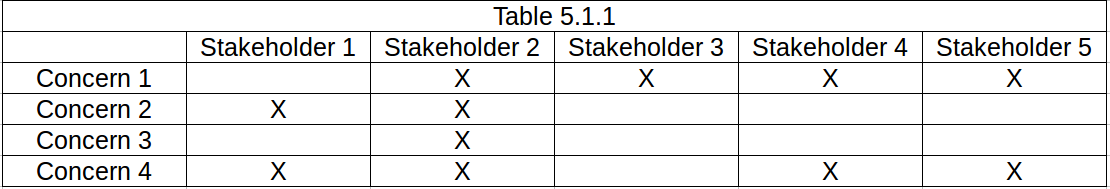
\includegraphics[width=140mm]{./trace.png}

\pagebreak

\section{Views}
%Listed below are views which.

\subsection{Logical View}
The Logical View focuses on realising the functionality of the FindMeTutor system.This view address the concerns of the end-user by realising the functionality of the system.\\\\
The FindMeTutor application uses a 2-Tier architecture.\\
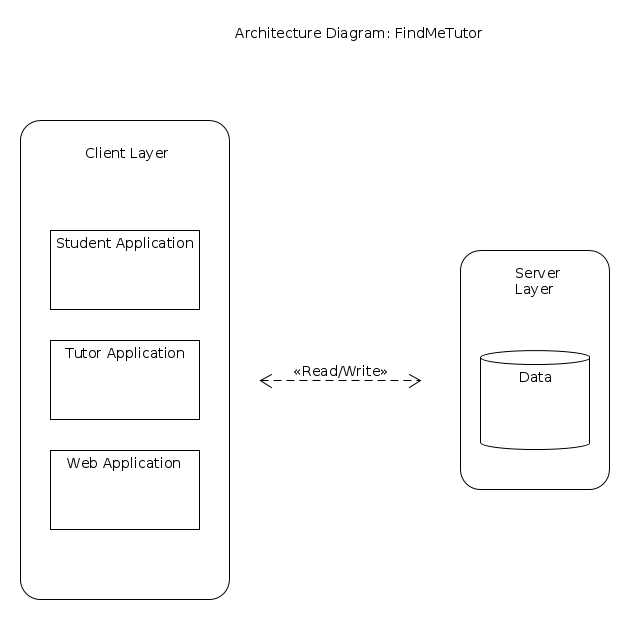
\includegraphics[width=140mm]{./architecture_diagram.png}
Put in diagram similar to above of sequence of how to request a tutor.\\

\subsubsection{Class Diagram}
The class diagram below describes the structure of the FindMeTutor system ny showing the system classes, their attributes and relationships to one another.\\
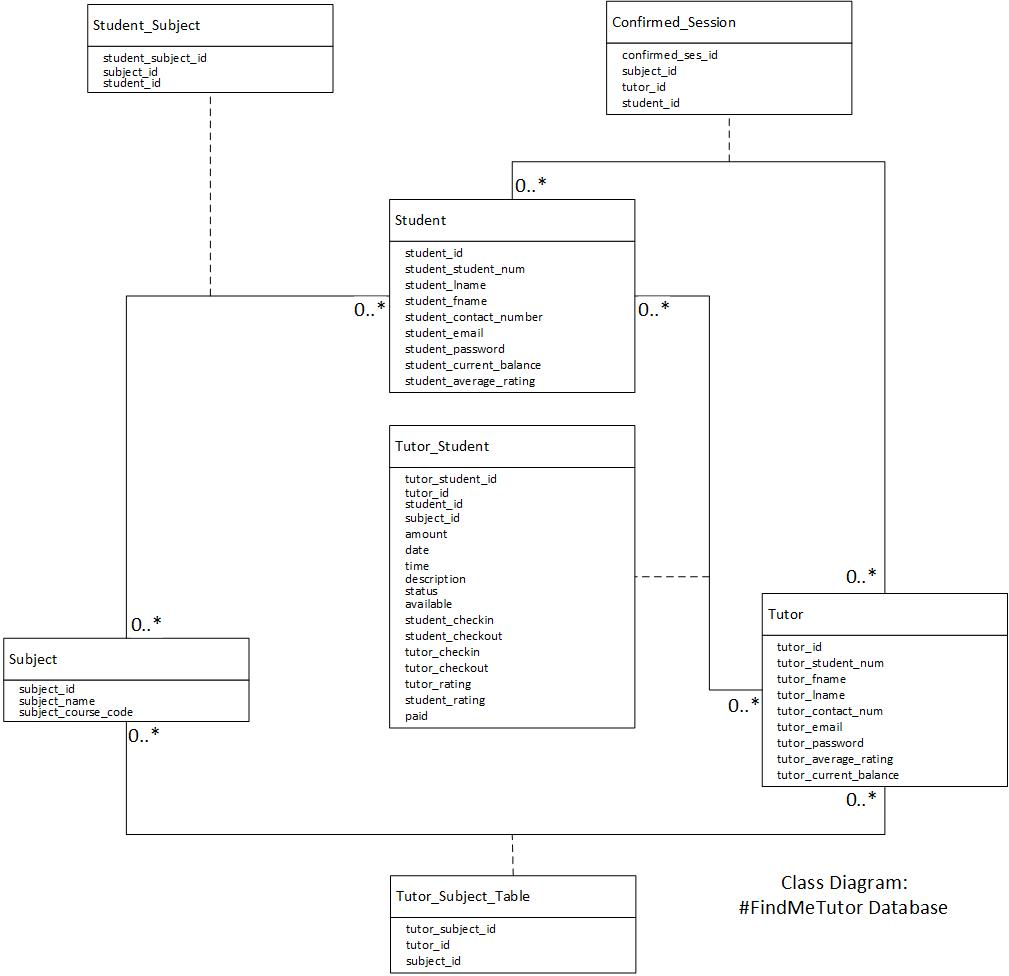
\includegraphics[width=140mm]{./class_diagram_findme_tutor.jpg}

\subsubsection{Sequence Diagram}
Sequence Diagrams show the sequence of messages passed between objects of the system over time.\\
\\\textbf{Create Student Sequence Diagram}:\\
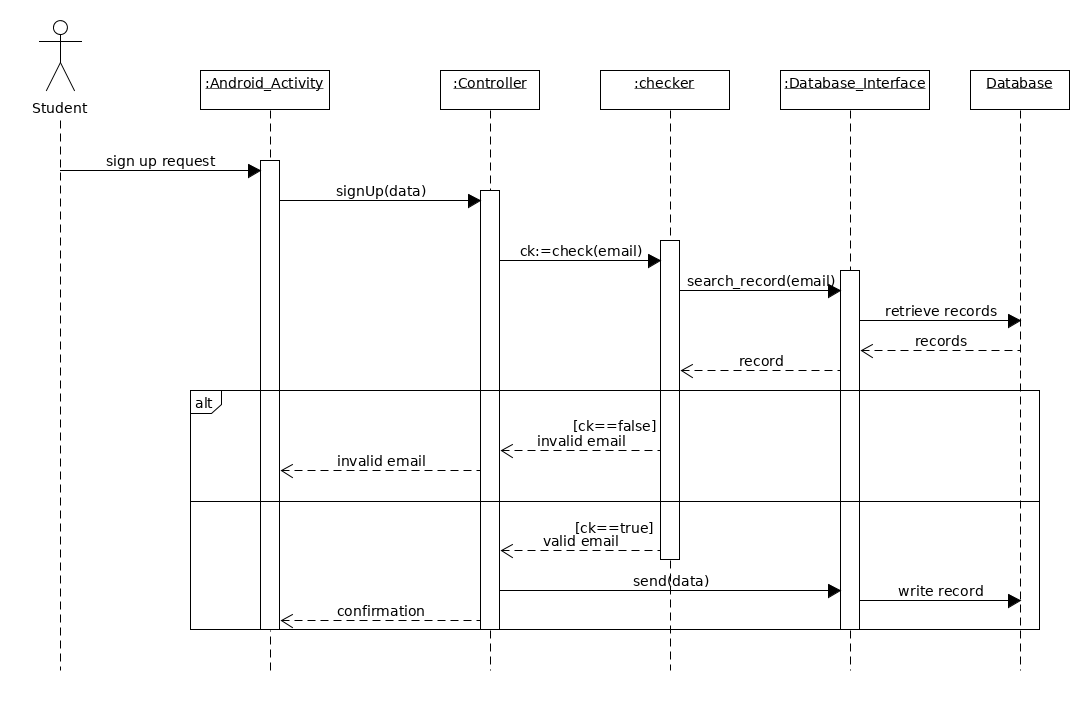
\includegraphics[width=140mm]{./sequence_diagram/create_student.png}
\textbf{Request Tutor Sequence Diagram}:\\
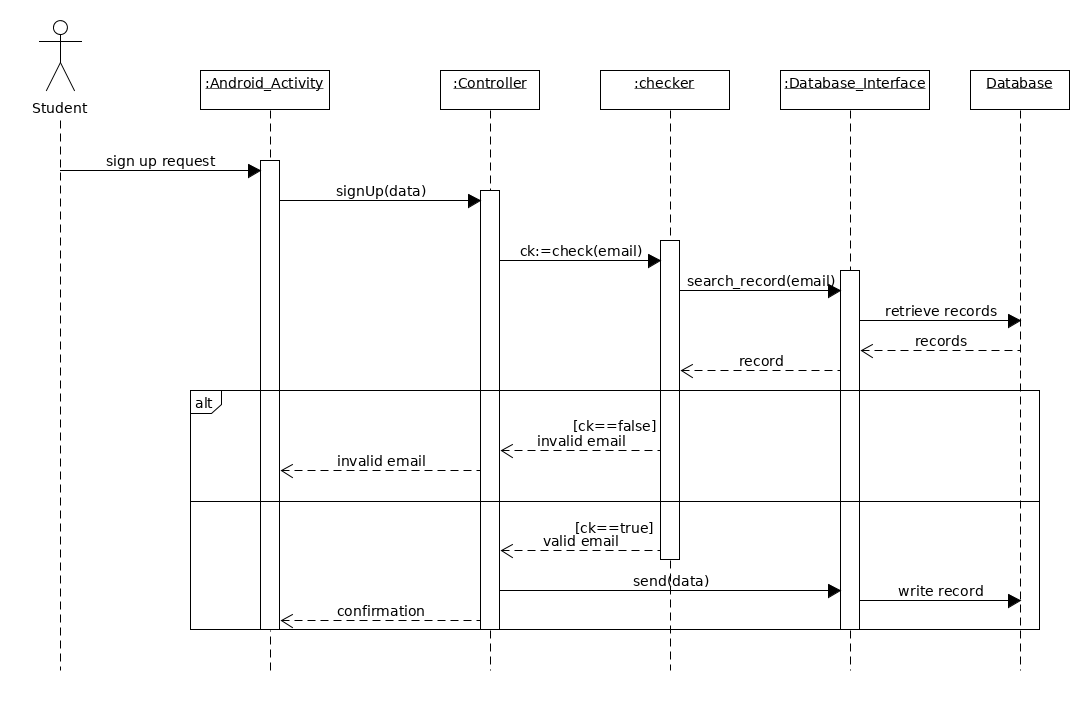
\includegraphics[width=140mm]{./sequence_diagram/request_tutor.png}
\textbf{Add Subject Sequence Diagram}:\\
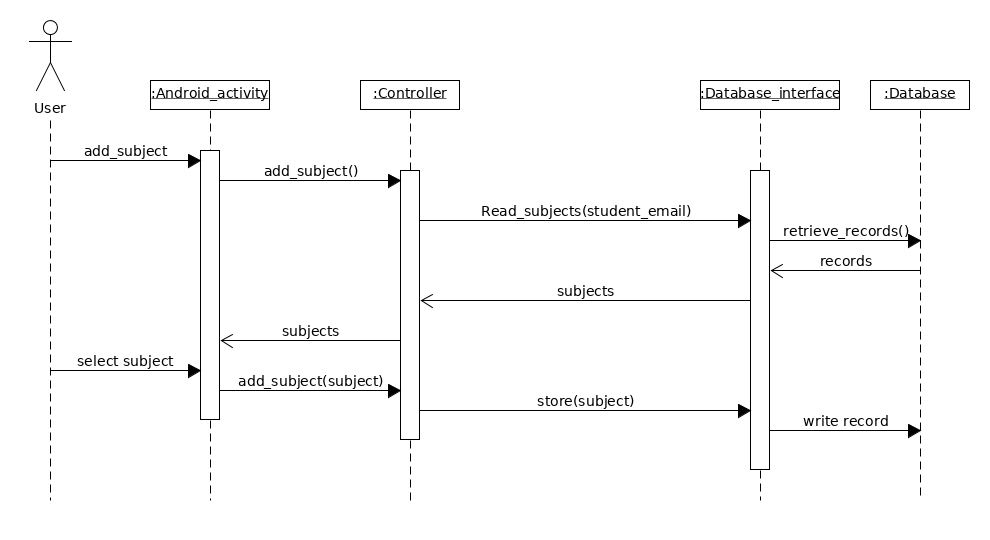
\includegraphics[width=140mm]{./sequence_diagram/add_subject.png}

\newpage

\subsection{Development View}
The Development view outlines the components that are used to assemble the physical system.
This view addresses the concerns of stakeholders concerned with the development of system such as developers.\\
\subsubsection{Package Diagram}

A package diagram depicts the dependencies the packages of the FindMeTutor system.
Below is package diagrams of the FindMeTutor system:\\
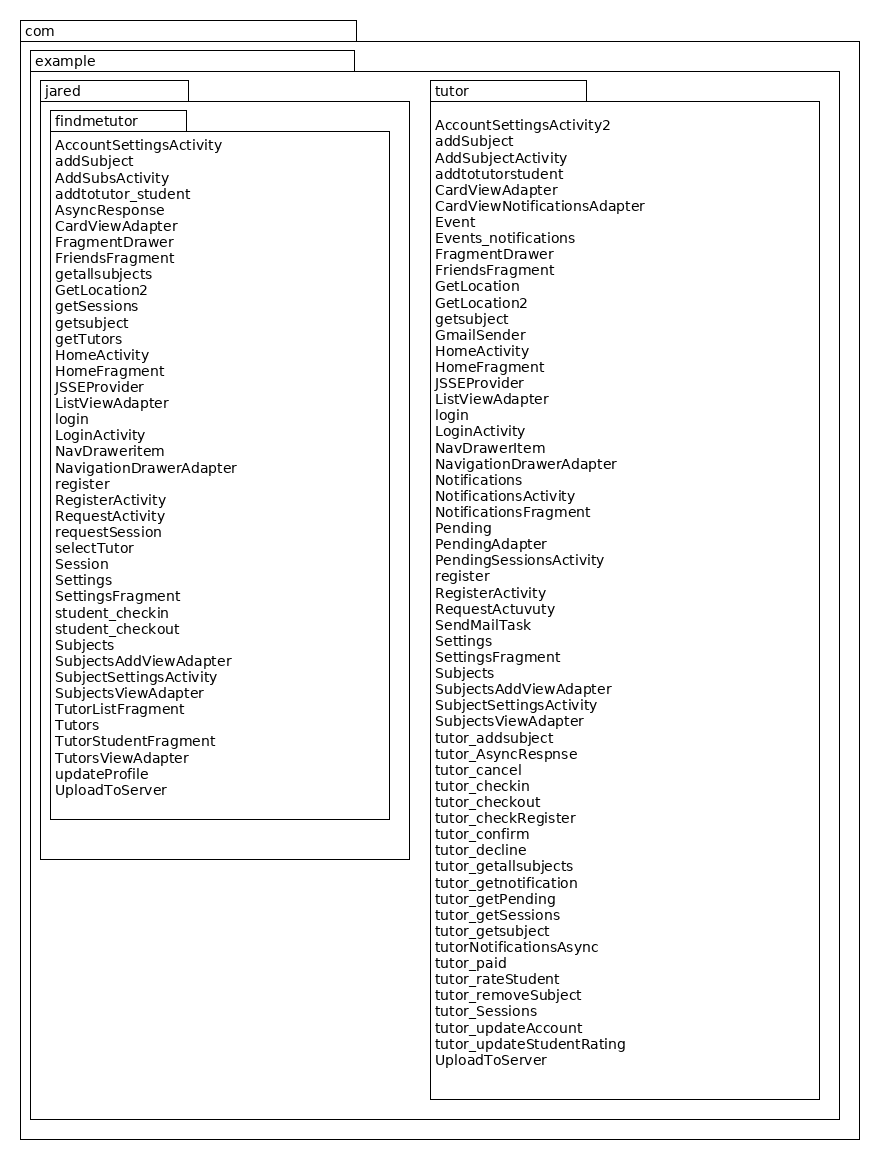
\includegraphics[width=140mm]{./package_diagram/package_diagram.png}


\subsubsection{Component Diagram}
A component diagram describes the components used to achieve the functionality of the system.\\
\textbf{ADD COMPONENT DIAGRAM}

\newpage

\subsection{Process View}
The process view considers the non-functional aspects of the system. It addresses the concerns of stakeholders concerned
with the design of the system.

\subsubsection{Activity Diagrams}
An activity diagram depicts the the flows of the system and business logic with actions.\\
\\\textbf{Request Tutor:}\\
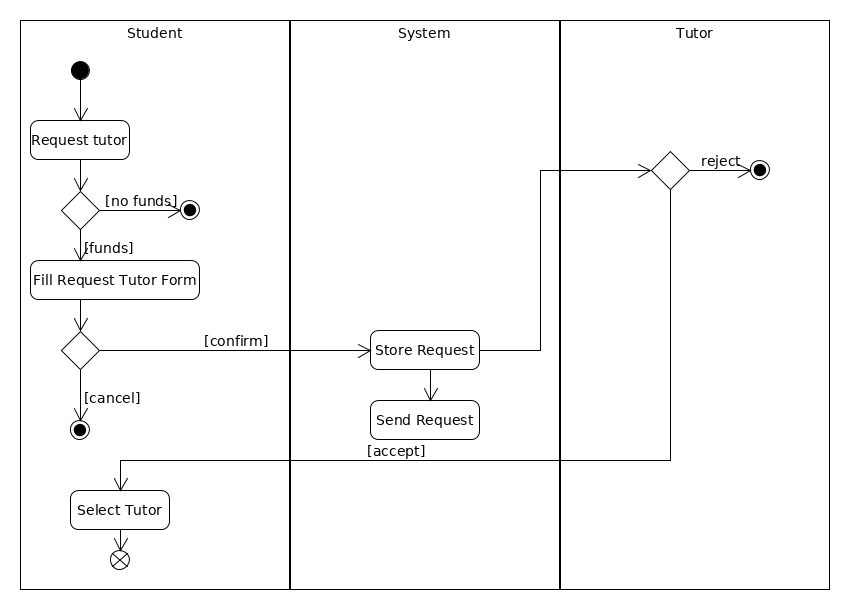
\includegraphics[width=140mm]{./activity_diagram/request_tutor.png}
\\\\\textbf{Check In:}\\
The initiating actor is either a student or a tutor where a participating actor refers to a tutor or student.\\
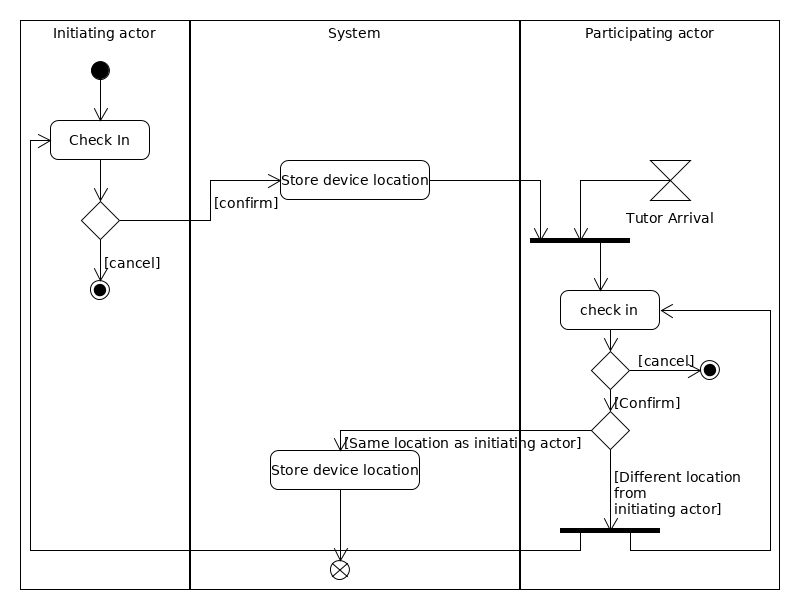
\includegraphics[width=140mm]{./activity_diagram/checked_in.png}
\\\\\textbf{Rate Tutor:}\\
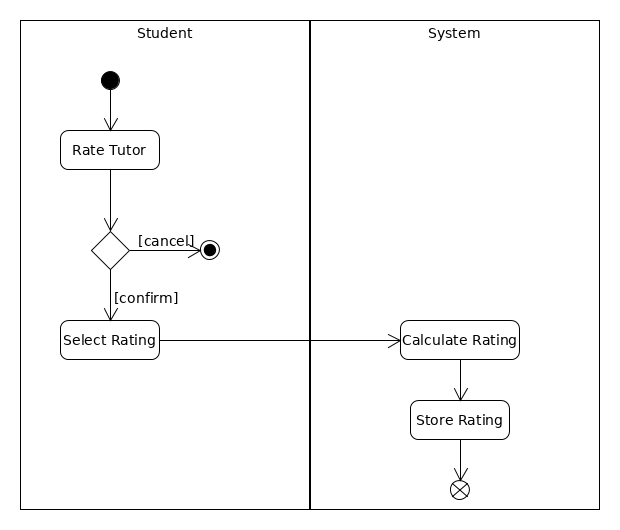
\includegraphics[width=140mm]{./activity_diagram/rate_tutor.png}

\newpage

\subsection{Physical View}
The physical view describes the physical locations of software, the scalability of the system, the deployment and installation.
\subsubsection{Deployment Diagram}

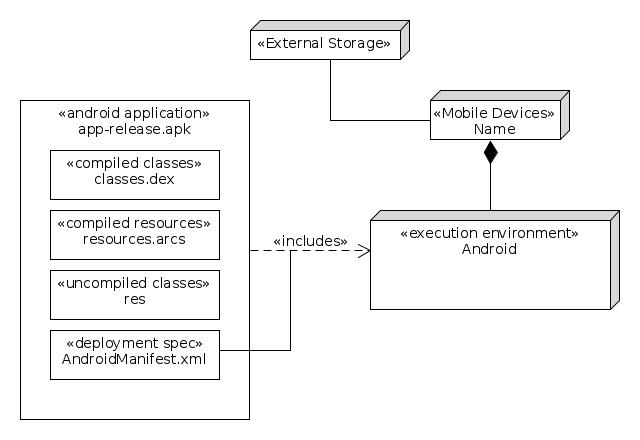
\includegraphics[width=140mm]{./Deployment.jpg}

\newpage

\subsection{Scenarios}
The Scenarios view address concerns of all stakeholders, this view helps show how the system is to be used.
\subsubsection{Use Case Diagram}
The use case diagram describes the behaviour of the system from the view of it's users.\\
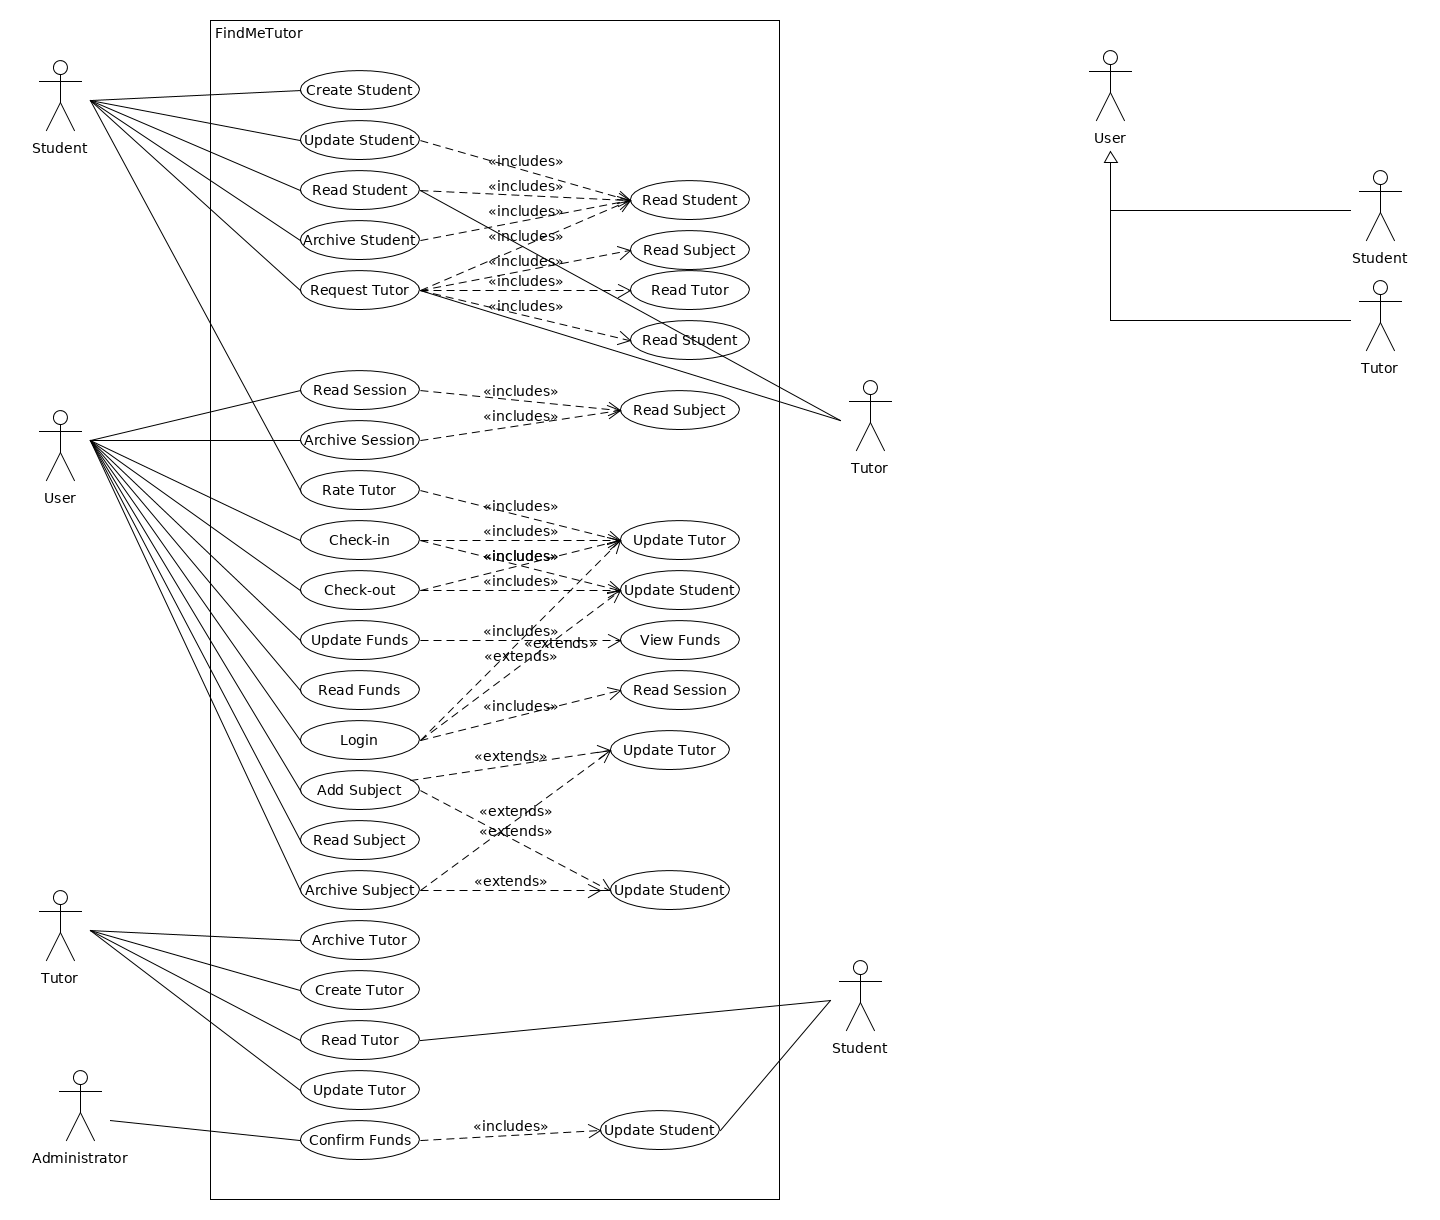
\includegraphics[width=170mm]{./Use_Case_Diagram.png}

\end{document}
